\documentclass[10pt]{beamer}

\usetheme{CambridgeUS}
\usepackage[english, russian]{babel}
\usepackage[utf8]{inputenc}
\usepackage{caption}
\usepackage{etoolbox}
\usepackage{multicol}
\usepackage{listings}
\usepackage{wasysym}
\usepackage{mathtools}
\DeclarePairedDelimiter\ceil{\lceil}{\rceil}
\DeclarePairedDelimiter\floor{\lfloor}{\rfloor}

\definecolor{mygreen}{rgb}{0,0.6,0}
\lstset{
  basicstyle=\ttfamily\footnotesize,        % the size of the fonts that are used for the code
  breaklines=true,                 % automatic line breaking only at whitespace
  captionpos=b,                    % sets the caption-position to bottom
  commentstyle=\color{mygreen},    % comment style
  keywordstyle=\color{blue},       % keyword style
  stringstyle=\color{red},     % string literal style
  showstringspaces=false,
  morekeywords={include, printf},
  texcl=true     %<---- added
}


\title[\href{https://goo.gl/NRgp8K}{https://goo.gl/NRgp8K} (Term 1)]{Сортировки}
\author[Гусев Илья, Булгаков Илья]{Гусев Илья, Булгаков Илья}
\institute[МФТИ] 
{Московский физико-технический институт\\*}
\date{Москва, 2018}
\subject{Computer Science}

\begin{document}

\begin{frame}
  \titlepage
\end{frame}

\begin{frame}{Содержание}
\tableofcontents
\end{frame}

\section{Задача}
\begin{frame}[fragile]{Задача сортировки}

Пусть требуется упорядочить N элементов: $R_{1},R_{2},\dots ,R_{n}$.\\
К - K - ключ сортировки, $\forall j \in 1\dots n, K_j \in R_j$\\
$\forall a, b, c \in K \rightarrow (a < b) \vee (b > a) \vee (a = b)$
$\forall a, b, c \in K \rightarrow (a < b) \wedge (b < c) \Rightarrow (a < c)$\\
Найти $p(1)p(2)\dots p(n)$ т.ч. $K_{p(1)}\leq K_{p(2)}\leq \dots \leq K_{p(n)}$\\
Устойчивая (стабильная) перестановка: $\forall i < j, K_{p(i)}=K_{p(j)} \rightarrow p(i)<p(j)$
\end{frame}

\section{Сортировка вставками}
\begin{frame}[fragile]{Сортировка вставками}
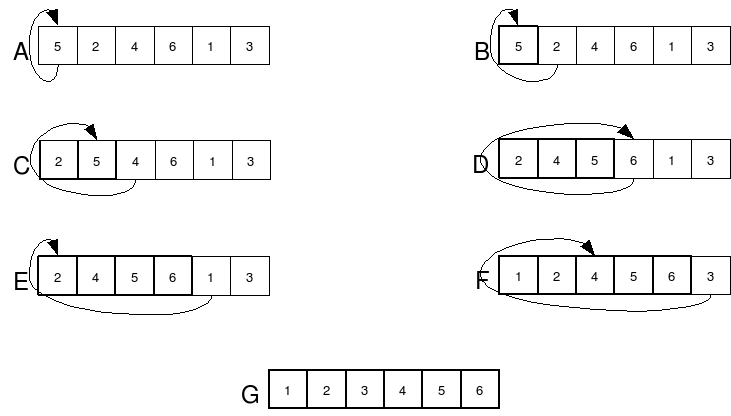
\includegraphics[width=11cm, height=6cm]{Term_1/Source/Pirctures/ins_sort.png}\\
Сложность? Устойчивость? Доп. память? Сложность на уже сортированных массивах? 
\end{frame}

\begin{frame}[fragile]{Сортировка вставками}{Код}
\begin{lstlisting}[language=C++]
template <class T>
void insertion_sort(std::vector<T>& collection) {
    for (size_t i = 1; i < collection.size(); i++) {
        T key = collection[i];
        size_t j = i - 1;
        while (j >= 0 && collection[j] > key) {
            collection[j + 1] = collection[j];
            j -= 1;
        }
        A[j+1] = key;
    }
}
\end{lstlisting}
\end{frame}

\section{Пирамидальная сортировка (HeapSort)}
\begin{frame}[fragile]{Пирамидальная сортировка (HeapSort)}
\begin{multicols}{2}
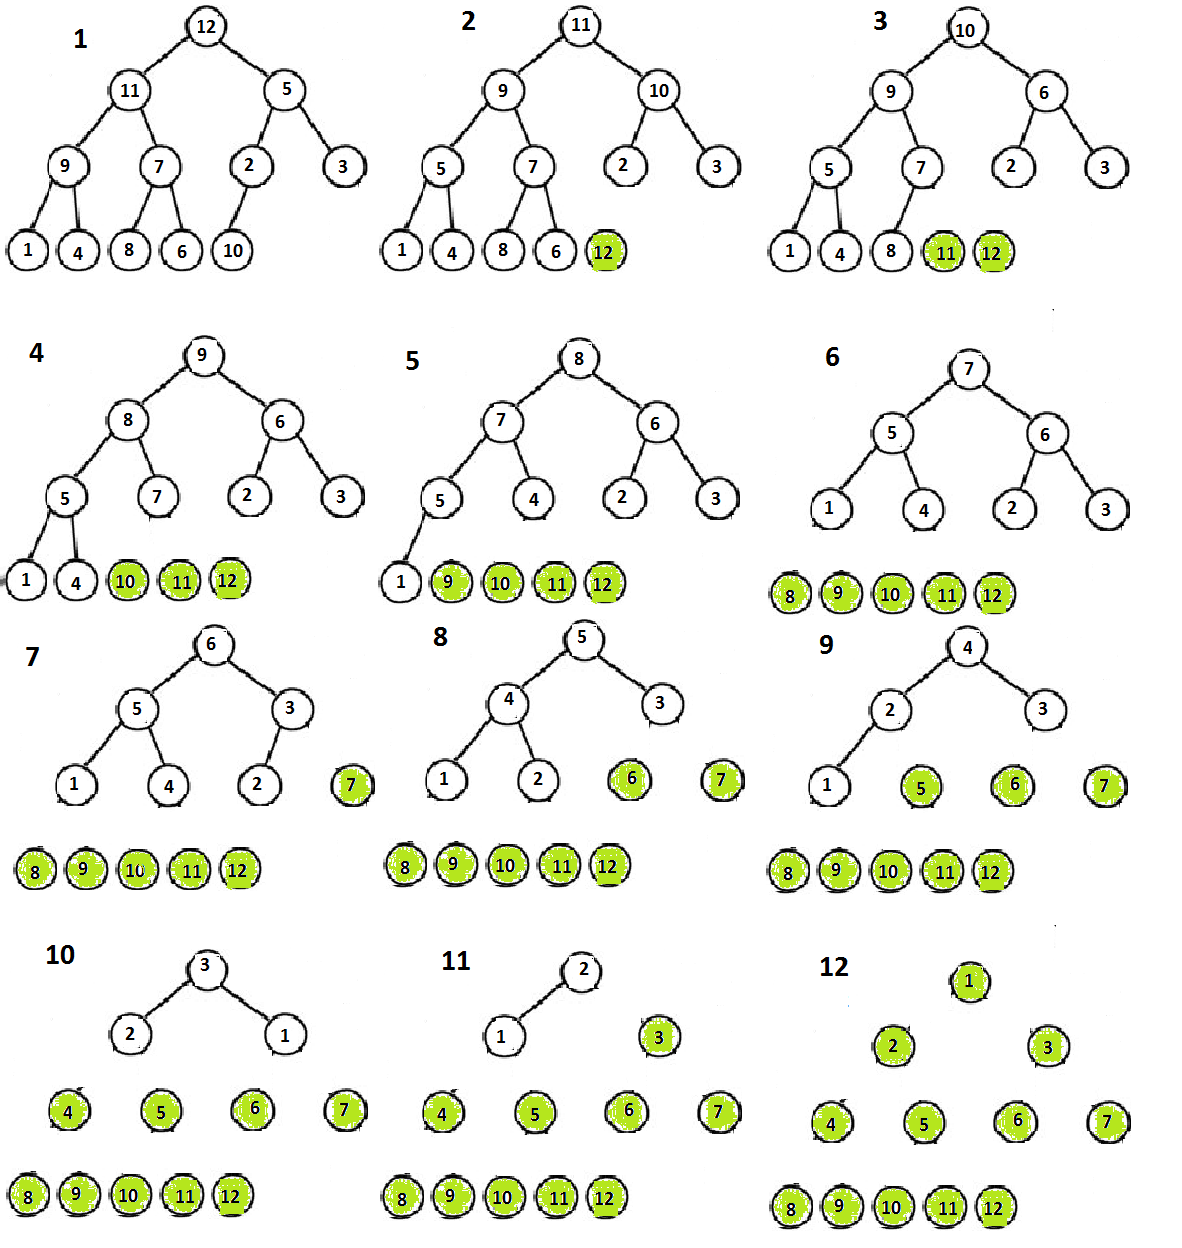
\includegraphics[width=6cm, height=6cm]{Term_1/Source/Pirctures/heapsort.png}\\
\vfill\eject
\begin{enumerate}
    \item Строим над коллекцией кучу
    \item Делаем ExtractMin n раз (минимум перемещаем в конец)
    \item ...
    \item PROFIT!
\end{enumerate}
Сложность? Устойчивость? Доп. память? Сложность на уже сортированных массивах? 
\end{multicols}
\end{frame}

\section{Сортировка слиянием (MergeSort)}
\begin{frame}[fragile]{Сортировка слиянием (MergeSort)}{Recursive}
\begin{multicols}{2}
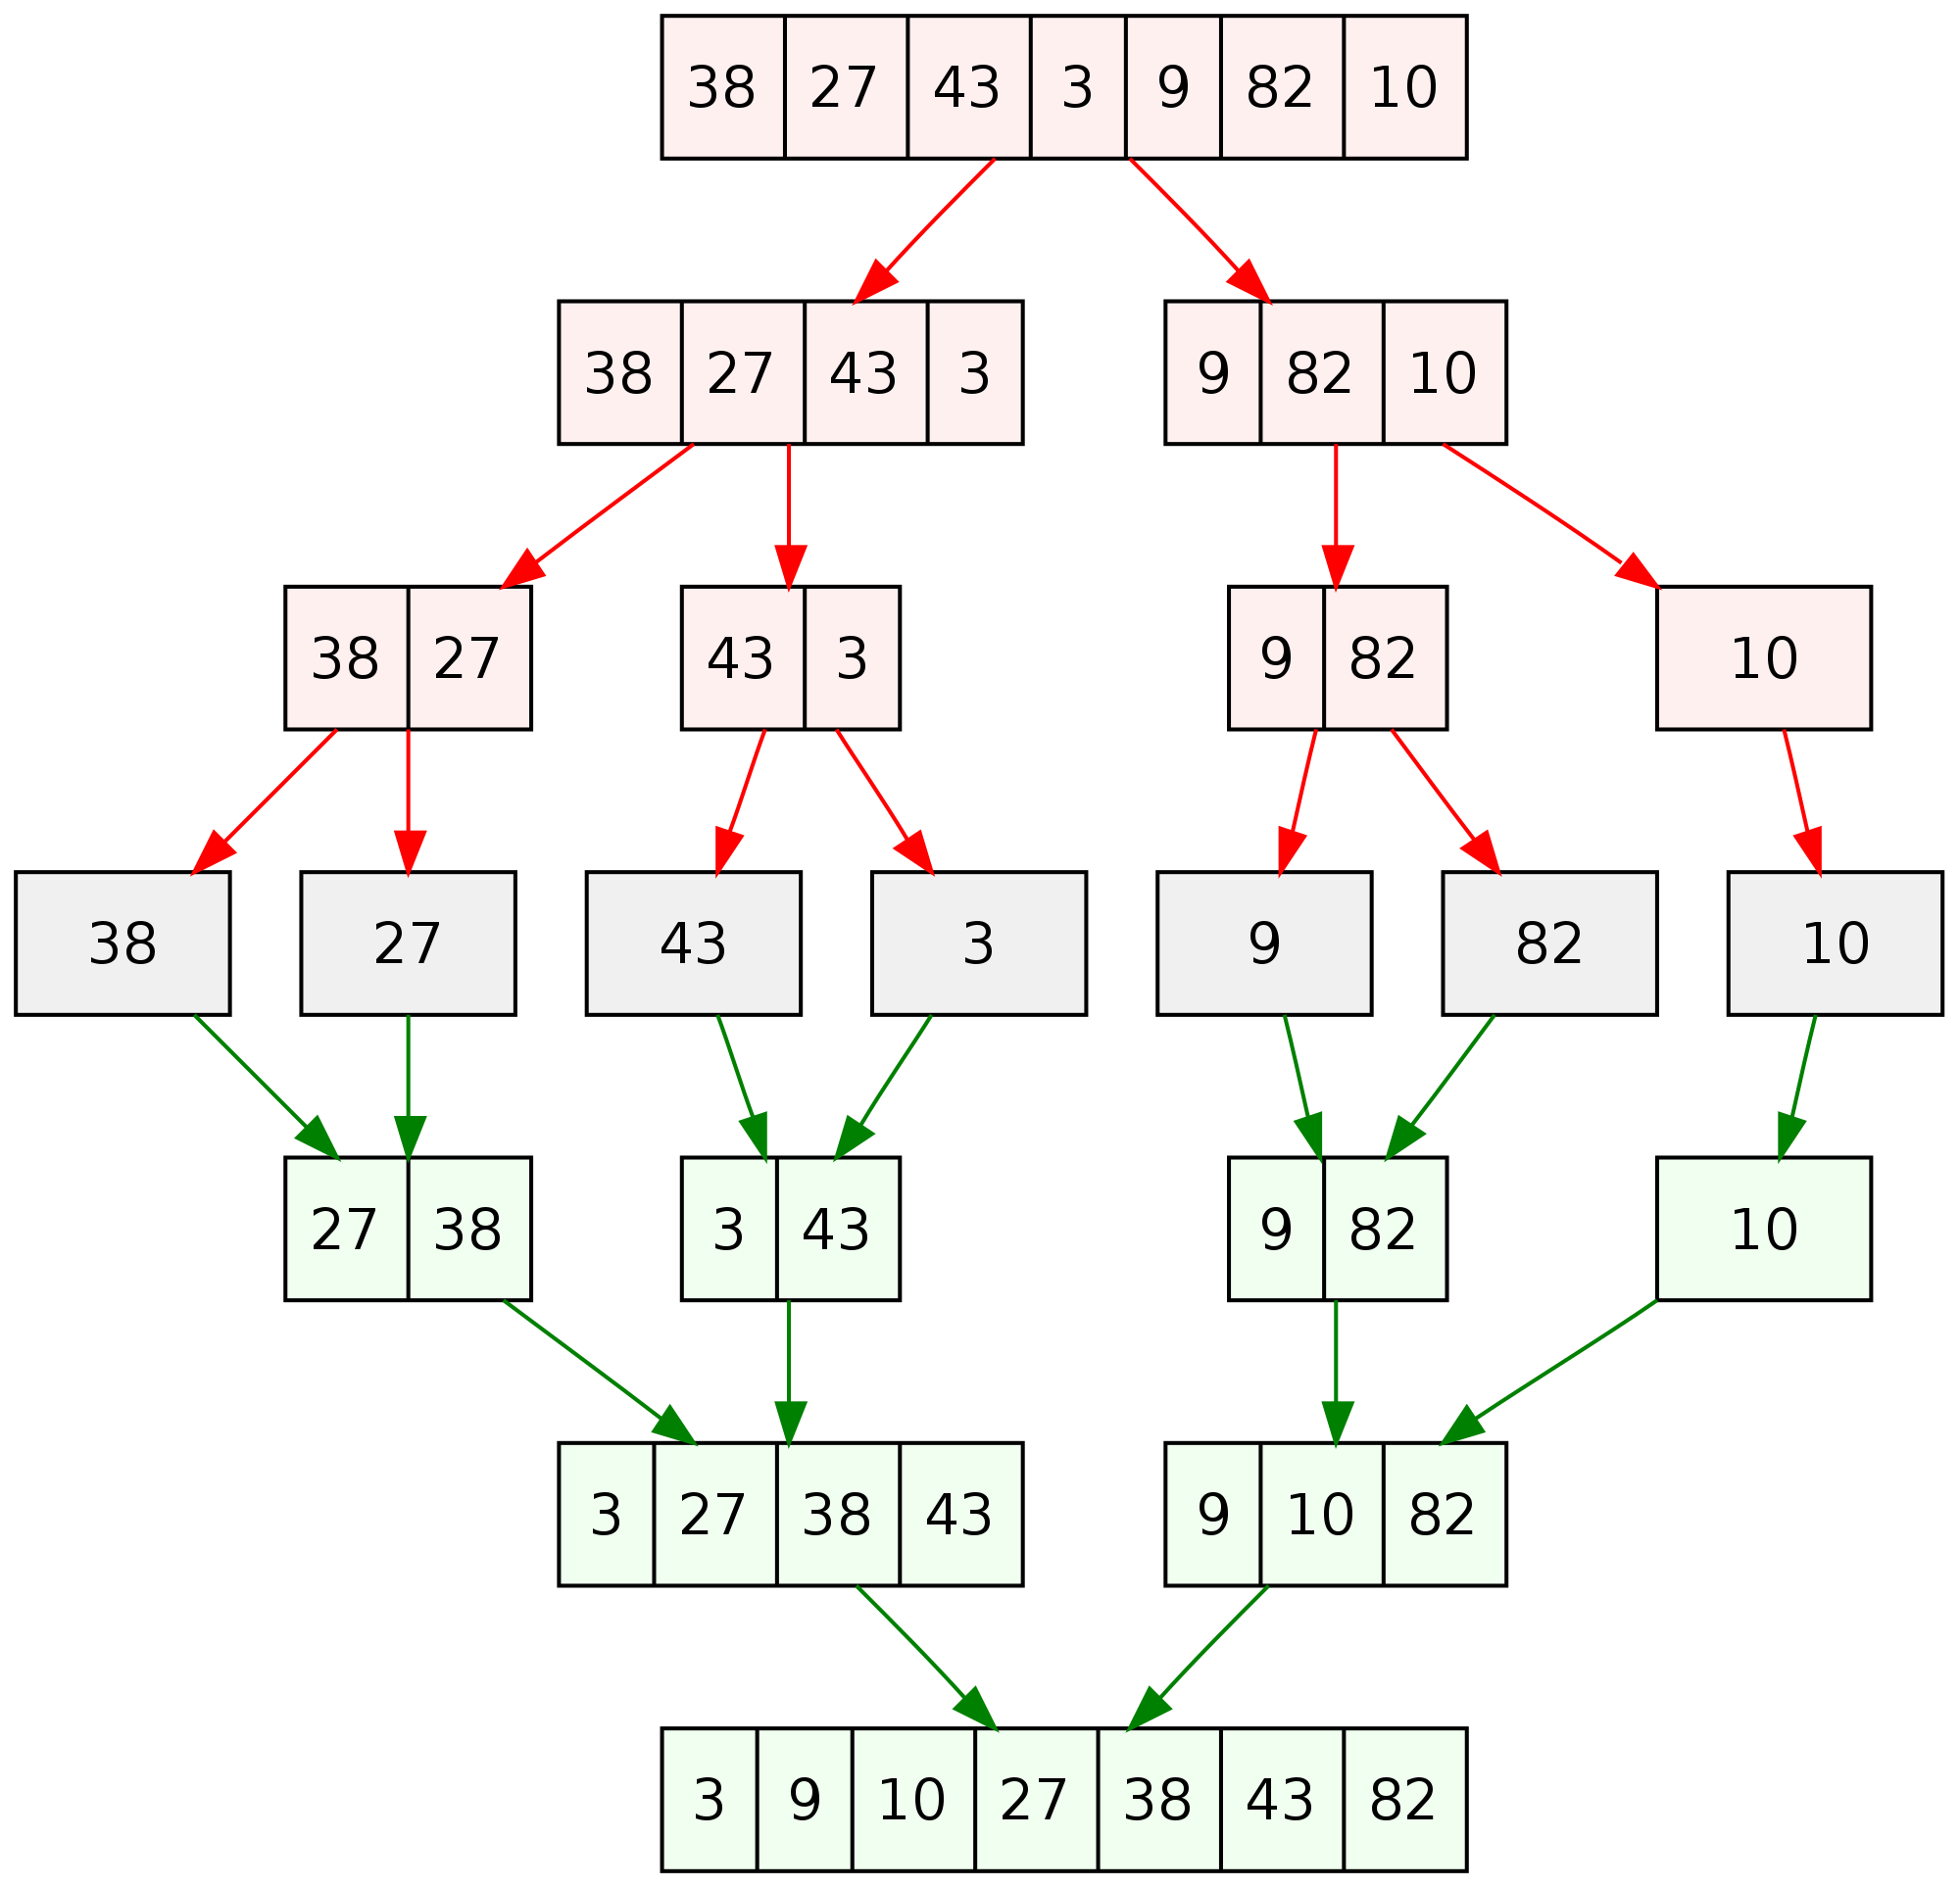
\includegraphics[width=6cm, height=6cm]{Term_1/Source/Pirctures/Merge_sort_algorithm.png}\\
\vfill\eject
Рекурсивный вариант
\begin{enumerate}
    \item Сортируемый массив разбивается на две части примерно одинакового размера
    \item Каждая из получившихся частей сортируется отдельно, например — тем же самым алгоритмом
    \item Два упорядоченных массива половинного размера соединяются в один
\end{enumerate}
\end{multicols}

\end{frame}

\begin{frame}[fragile]{Сортировка слиянием (MergeSort)}{Merge}
\begin{multicols}{2}
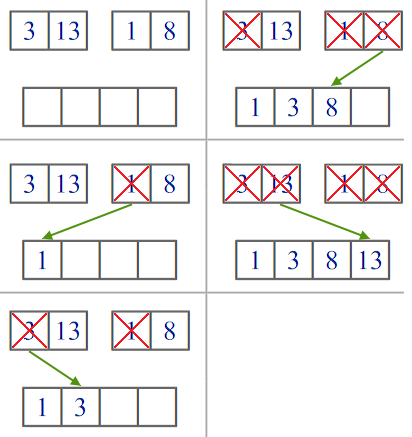
\includegraphics[width=6cm, height=6cm]{Term_1/Source/Pirctures/Merging_two_arrays.png}\\
\vfill\eject
\begin{itemize}
    \item Время работы процедуры: $\Theta(m)$, где m - суммарное количество входных данных
    \item Суммарно для всех вызовов на одном уровне: $\Theta(n)$, где n - количество элементов коллекции
\end{itemize}
\end{multicols}
\end{frame}

\begin{frame}[fragile]{Сортировка слиянием (MergeSort)}{Iterative}
\begin{multicols}{2}
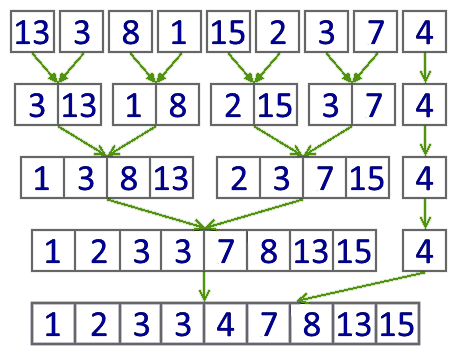
\includegraphics[width=6cm, height=4.6cm]{Term_1/Source/Pirctures/Merge_sort_itearative.png}\\
\vfill\eject
\begin{itemize}
    \item Альтернатива: итеративный алгоритм
    \item Сложность? Устойчивость? Доп. память? Сложность на уже сортированных массивах? 
\end{itemize}
\end{multicols}
\end{frame}

\section{Быстрая сортировка (QuickSort)}
\begin{frame}[fragile]{Быстрая сортировка (QuickSort)}{Partition}
\begin{multicols}{2}
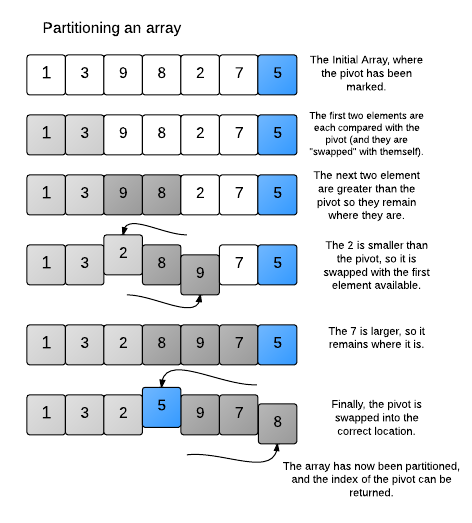
\includegraphics[width=6cm, height=6cm]{Term_1/Source/Pirctures/qs1.png}\\
\vfill\eject
\begin{itemize}
    \item Сделать Partition коллекции
    \item Partition - берём опорный элемент, а остальные элементы делим на две части: меньше опорного и больше или равные опорному. $\Theta(n)$
    \item Для обоих частей рекурсивно выполняем Partition
    \item Тип Partition: Хоара или Ломуто
\end{itemize}
\end{multicols}
\end{frame}

\begin{frame}[fragile]{Быстрая сортировка (QuickSort)}
Сложность? Устойчивость? Доп. память? Сложность на уже сортированных массивах?\\
Модификации:

\begin{itemize}
    \item Устойчивость через второй ключ-индекс
    \item Выбор опорного элемента: первый, последний, средний, медианный из 3, случайный
    \item Разбиение на 3 части
\end{itemize}
\end{frame}

\section{Сравнение сортировок}
\begin{frame}[fragile]{Сравнение сортировок}
\begin{table}
\small
\begin{tabular}{ |c|c|c|c|c|c|c|} 
 \hline
Алгоритм & Худшее & Лучшее & В среднем & Sorted & Уст. & $+$ память \\
 \hline
Insertion & $\Theta(n^2)$ & $\Theta(n)$ & $\mathcal{O}(n^2)$ & $\Theta(n)$ & Да &  $\Theta(1)$\\
 \hline
Heap & $\Theta(nlog(n))$ & $\Theta(nlog(n))$ & $\Theta(nlog(n))$ & $\Theta(nlog(n))$ & Нет &  $\Theta(1)$\\
 \hline
Merge & $\Theta(nlog(n))$ & $\Theta(nlog(n))$ & $\Theta(nlog(n))$ & $\Theta(nlog(n))$ & Да &  $\Theta(n)$\\
 \hline
Quick & $\Theta(n^2)$ & $\Theta(nlog(n))$ & $\Theta(nlog(n))$ & $\Theta(n^2)$ & Нет &  $\Theta(1)$\\
 \hline
\end{tabular}
\end{table}
\end{frame}

\section{Доказательство $\Omega(nlog(n))$ для сортировок сравнениями}
\begin{frame}[fragile]{Доказательство $\Omega(nlog(n))$ для сортировок сравнениями}
\begin{multicols}{2}
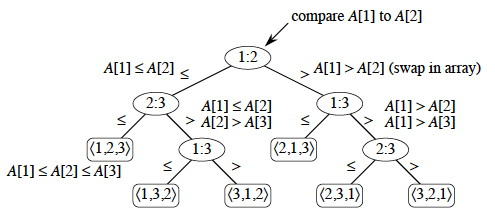
\includegraphics[width=6cm, height=3.1cm]{Term_1/Source/Pirctures/decision-tree-insertion-sort.jpg}\\
\vfill\eject
\begin{itemize}
    \item $count(leaves) = l \geq n!$
    \item $l \leq 2^h$
    \item $n! \leq l \leq 2^h \Rightarrow log_2(n!) \leq h$
    \item $n! > (\frac{n}{e})^n$
    \begin{itemize}
        \item $1 > \frac{1}{e}$
        \item $(\frac{n+1}{e})^{n+1} = (\frac{n}{e})^n \frac{(n+1)^{n+1}}{n^n e} = (\frac{n}{e})^n (1+\frac{1}{n})^n \frac{n+1}{e} > n! (n+1) = (n+1)!$
    \end{itemize}
    \item $h \geq log_2(\frac{n}{e})^n = n \cdot log_2(\frac{n}{e}) = \Omega(n \cdot log(n))$
\end{itemize}
\end{multicols}
\end{frame}


\appendix
\section<presentation>*{\appendixname}
\subsection<presentation>*{Useful links}

\begin{frame}[allowframebreaks]
  \frametitle<presentation>{Полезные ссылки}
    
  \begin{thebibliography}{10}
{
  \beamertemplatearticlebibitems
  
  \bibitem{ICS}
  \texttt{ICS 311 \#10: Theoretical Limits of Sorting, O(n) Sorts}
  \newblock \href{https://www2.hawaii.edu/\~nodari/teaching/s17/Notes/Topic-10.html}{\texttt{https://www2.hawaii.edu/\~nodari/teaching/s17/Notes/Topic-10.html}}
  
  \bibitem{Wiki}
  \texttt{Wiki - Sorting algorithm}
  \newblock \href{https://en.wikipedia.org/wiki/Sorting\_algorithm}{\texttt{https://en.wikipedia.org/wiki/Sorting\_algorithm}}
  
    
  \bibitem{neerc1}
  \texttt{Викиконспекты: Сортировка слиянием}
  \newblock \href{https://bit.ly/2DH6XmF}{\texttt{https://neerc.ifmo.ru/wiki/index.php?title=Сортировка_слиянием}}
  


}


  \end{thebibliography}
\end{frame}

\end{document}


